% Included from both -slides and -handout versions.

\mode<presentation>
{
  \usetheme{default}
  \useoutertheme{infolines}
}

\usepackage[english]{babel}
\usepackage[latin1]{inputenc}
\usepackage{graphicx}
\usepackage{times}
\usepackage[T1]{fontenc}
\usepackage{fancyvrb}
\usepackage{hyperref}
\usepackage{listings}
\begin{document}
\lstset{language=C, escapeinside={(*@}{@*)}, numbers=left,
  basicstyle=\tiny, showspaces=false, showtabs=false}

\title{L41: Lab 2 - IPC}
\author{Dr Robert N. M. Watson}
\date{5 November 2015}

\begin{frame}
  \titlepage
\end{frame}

\section{Introduction}

\begin{frame}
  \frametitle{L41: Lab 2 - Kernel implications of IPC}

  \begin{itemize}
    \item A quick note on \texttt{vm\_fault()}
    \item Learn about (and trace) POSIX IPC
    \item Explore buffering and scheduler interactions
    \item Measure the probe effect
    \item Start to gather data for assessed \textit{Lab Report 2}
  \end{itemize}
\end{frame}

\begin{frame}
  \frametitle{Recall: A (kernel) programmer model for VM}

  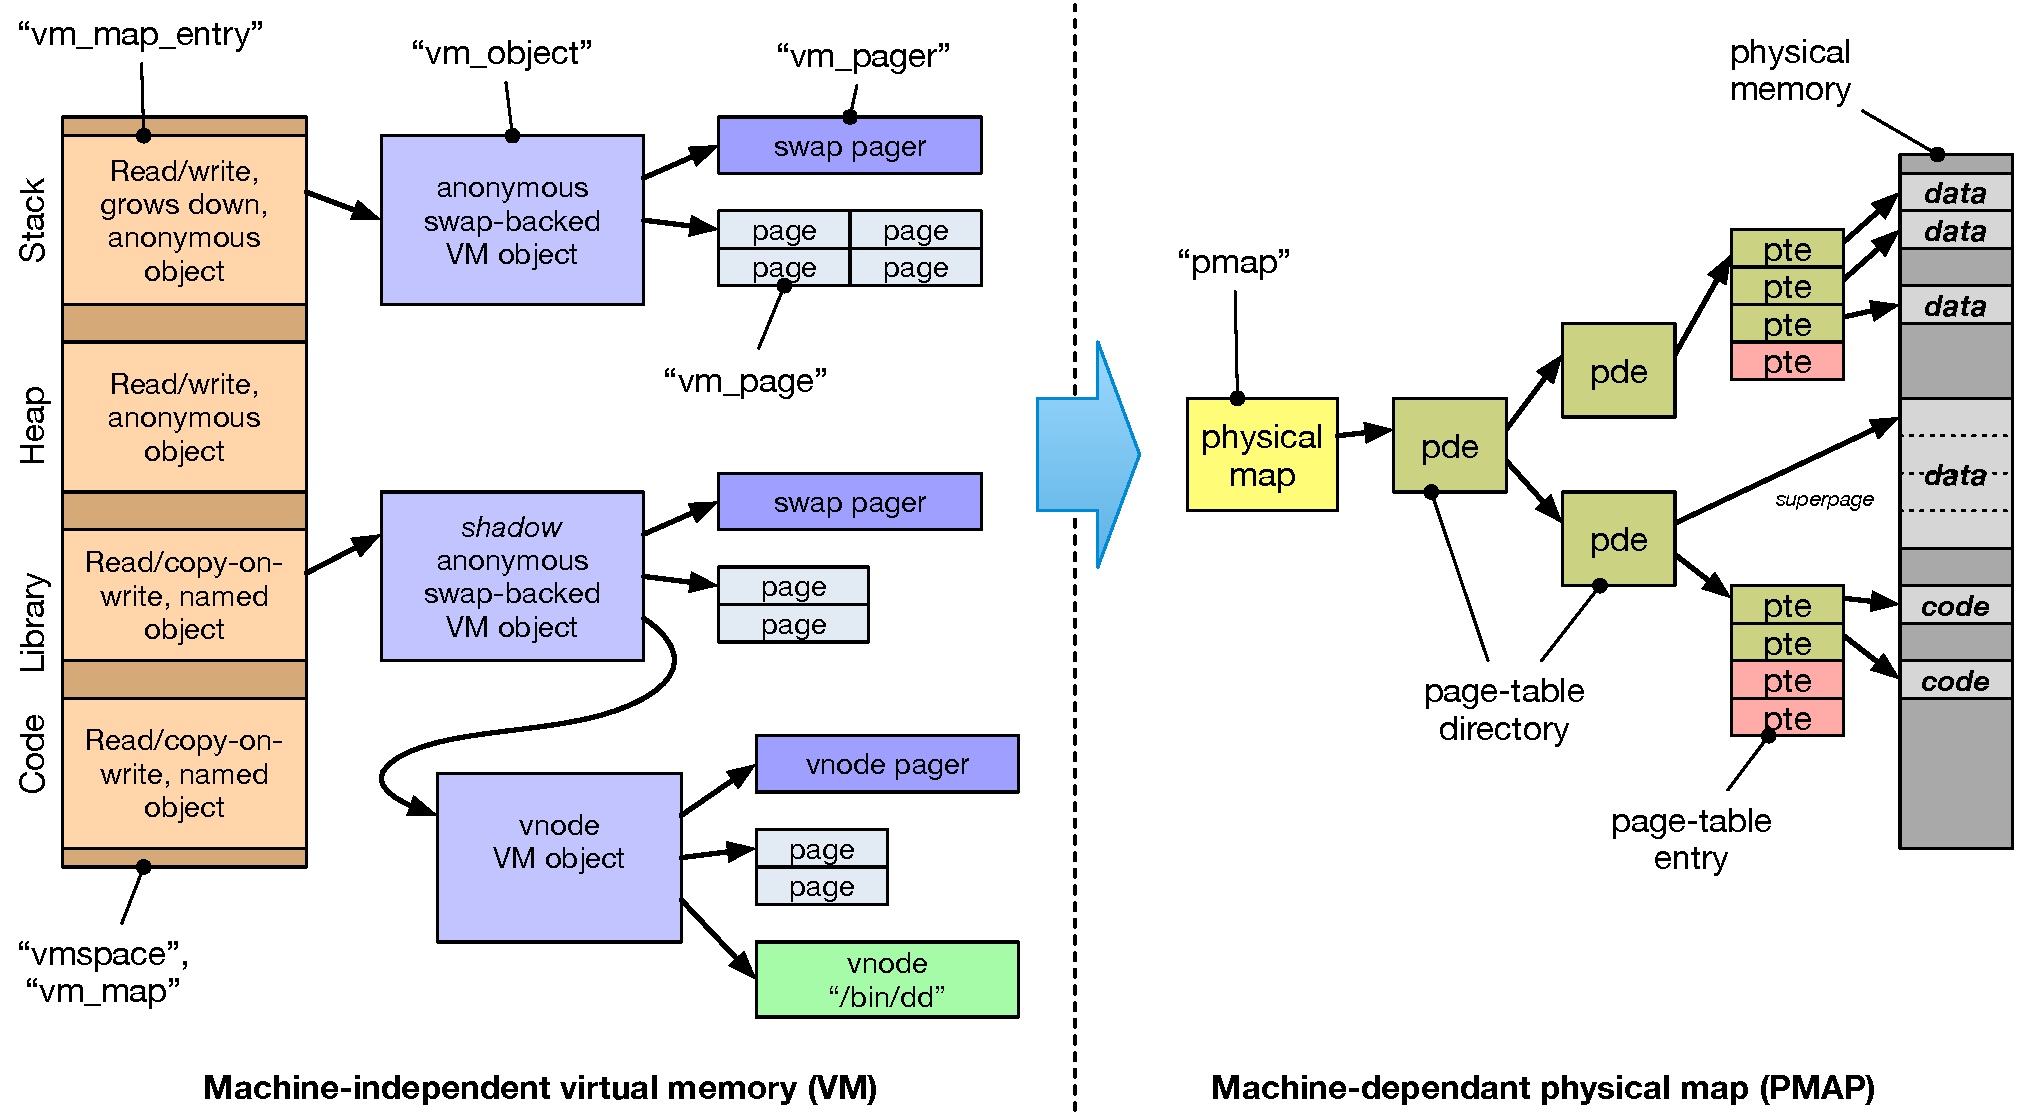
\includegraphics[width=\textwidth]{../../figures/mach-vm-model.pdf}
\end{frame}

\begin{frame}
  \frametitle{The Mach VM fault handler (\texttt{vm\_fault})}

  \begin{itemize}
    \item Key goal of the Mach VM system: be as lazy as possible
    \begin{itemize}
      \item Fill pages (with file data, zeroes, COW) on demand
      \item Map pages into address spaces on demand
      \item Flush TLB as infrequently as possible
    \end{itemize}
    \item Any work avoided means reduced CPU cycles and less disk I/O
    \item Avoid as much work as possible when creating a mapping \\
      (e.g., \texttt{mmap()}, \texttt{execve()})

    \pause
    \bigskip
    \item Instead, do on-demand in the MMU trap handler, \texttt{vm\_fault()}
    \begin{itemize}
      \item Machine-independent function drives almost all VM work
      \item Input: faulting virtual address, output mapped page or signal
      \item Look up object to find cached page; if none, invoke pager
      \item May trigger behaviour such as zero filling or copy-on-write
    \end{itemize}

    \pause
    \bigskip
    \item A good thing to probe with DTrace to understand VM traps
  \end{itemize}
\end{frame}

\begin{frame}[fragile]
  \frametitle{The benchmark}

  \begin{scriptsize}
\begin{verbatim}
[guest@beaglebone ~/ipc] ./ipc-static 
ipc-static [-Bqsv] [-b buffersize] [-i pipe|local] [-t totalsize] mode

Modes (pick one - default 1thread):
    1thread         IPC within a single thread
    2thread         IPC between two threads in one process
    2proc           IPC between two threads in two different processes

Optional flags:
    -B              Run in bare mode: no preparatory activities
    -i pipe|local   Select pipe or socket for IPC (default: pipe)
    -q              Just run the benchmark, don't print stuff out
    -s              Set send/receive socket-buffer sizes to buffersize
    -v              Provide a verbose benchmark description
    -b buffersize   Specify a buffer size (default: 131072)
    -t totalsize    Specify total I/O size (default: 16777216)
\end{verbatim}
  \end{scriptsize}

  \begin{itemize}
    \item Simple, bespoke IPC benchmark: pipes and sockets
    \item Statically or dynamically linked
    \item Adjust user and kernel buffer sizes
    \item Various output modes
  \end{itemize}
\end{frame}

\begin{frame}
  \frametitle{The benchmark (2)}

  \begin{itemize}
    \item Three operational modes:
    \begin{description}
      \item[1thread] IPC within a single thread of a single process
      \item[2thread] IPC between two threads of a single process
      \item[2proc] IPC between two threads in two processes
    \end{description}
    \pause
    \item Adjust IPC parameters:
    \begin{description}
      \item[\texttt{-i pipe}] Use \texttt{pipe()} IPC
      \item[\texttt{-i local}] Use \texttt{socketpair()} IPC
      \item[\texttt{-b size}] Set user IPC buffer size
      \item[\texttt{-t size}] Set total size across all IPCs
      \item[\texttt{-s}] Also set in-kernel buffer size for sockets
      \item[\texttt{-B}] Suppress quiescence (whole-program tracing)
    \end{description}
    \pause
    \item Output flags:
    \begin{description}
      \item[\texttt{-q}] Suppress all output (whole-program tracing)
      \item[\texttt{-v}] Verbose output (interactive testing)
    \end{description}
  \end{itemize}
\end{frame}

\begin{frame}[fragile]
  \frametitle{The benchmark (3)}

  \begin{small}
\begin{verbatim}
[guest@beaglebone ~/ipc]$ ./ipc-static -v -i pipe 1thread
Benchmark configuration:
  buffersize: 131072
  totalsize: 16777216
  blockcount: 128
  mode: 1thread
  ipctype: pipe
  time: 0.033753791
485397.29 KBytes/sec
\end{verbatim}
  \end{small}

  \begin{itemize}
    \item Use verbose output
    \item Use pipe IPC
    \item Run benchmark in a single thread
    \item Use default \texttt{buffersize} of 128K, \texttt{totalsize} of 16M
  \end{itemize}
\end{frame}

\begin{frame}
  \frametitle{Exploratory questions -- baseline performance}

  \begin{enumerate}
    \item How do the various benchmark configurations perform?
    \item How do return values from \texttt{read()} and \texttt{write()} vary?
    \item How does setting the socket-buffer size impact performance?
    \item How much time do pipes vs. sockets spend in system calls?
    \item How do context-switch rates vary across configurations?
  \end{enumerate}
\end{frame}

\begin{frame}
  \frametitle{Experimental questions for the lab report}

  The full lab-report assignment will be distributed during the next lab.

  \medskip

  These questions are intended to help you gather data that you will need for
  that lab report:

  \begin{itemize}
    \item How does changing the buffer size affect IPC performance?
      For sockets, consider both with, and without, the \texttt{-s} flag.

    \item Is using multiple threads faster or slower than using multiple
      processes?
  \end{itemize}
\end{frame}

\begin{frame}
  \frametitle{This lab session}

  Use this session to continue to build experience:

  \begin{itemize}
    \item Build and use the IPC benchmark
    \item Use DTrace to analyse distributions of system calls, system-call
      execution times, and system-call arguments and return values
    \item Use \texttt{ministat} (or R, Python, ...) to analyse benchmark results
  \end{itemize}

  Do ask us if you have any questions or need help
\end{frame}

\end{document}
